\section{Test der Matrizenmultiplikation}
Zunächst wurde die Berechnung als Ganzzahl-Multiplikation mit dem Faktor 3 betrachtet. Da es bei diesem Faktor und den gewählten Eingangswerten nicht zu einem 
Überlauf kommen kann, war es zu diesem Zeitpunkt noch nicht nötig, sich Gedanken über die Breite des Ergebnisvektors bzw den Ausschnitt daraus für die weitere
Berechnung zu machen. Auch konnte an dieser Stelle noch auf den Bitshift zur Halbierung der Werte verzichtet werden.

Erst als der Faktor $\frac{\sqrt{2}}{2}$ übernommen wurde, wurden die Ergebnisse breiter als der Vektor für die weitere Berechnung an Bits zur Verfügung stellt.
Daraus folgt, dass ein Teil der Bits abgeschnitten werden müssen. Da die Dualzahlen jetzt im S1Q10-Format betrachtet werden, es sich also um Kommazahlen handelt,
müssen die hinteren Bits abgeschnitten werden. Zudem können vorne Bits ohne Informationsverlust gestrichen werden, da durch die Multiplikation ein weiteres 
Negations-Bit dazugekommen ist und auf Grund des gegebenen Faktors der Wertebereich vorne nie ganz ausgenutzt wird. (Verifizieren / Belegen!)


\section{Implementierung des Konstantenmultiplizieres}

Anfangs wurde angenommen, dass Multiplikationen mit den Twiddlefaktoren $\pm 1$ und $\pm\frac{\sqrt{2}}{2}$ durchgeführt werden müssen. 
Dass bei einer optimierten 8x8-DFT wegen des explizieten ausprogrammierens der Berechnungen die Multiplikation mit $\pm1$ wegfällt, wurde recht schnell klar.
Erst bei genauer Betrachtung der Twiddlefaktor-Matrix viel auf, dass in jeder Zeile gleich viele Additionen wie Subtraktionen vorhanden sind. Durch Umsortieren 
ist es dadurch möglich auf das Invertieren der Eingangswerte sowie den hierfür benötigten Takt und die Inverter zu verzichten. Weiter wird auch nur die Multiplikation
mit $+\frac{\sqrt{2}}{2}$ benötigt.

\subsection{Syntheseergebnis eines 12 Bit Kostantenmultiplizierers}
\begin{figure}[!ht]
\centering  
 \fbox{
  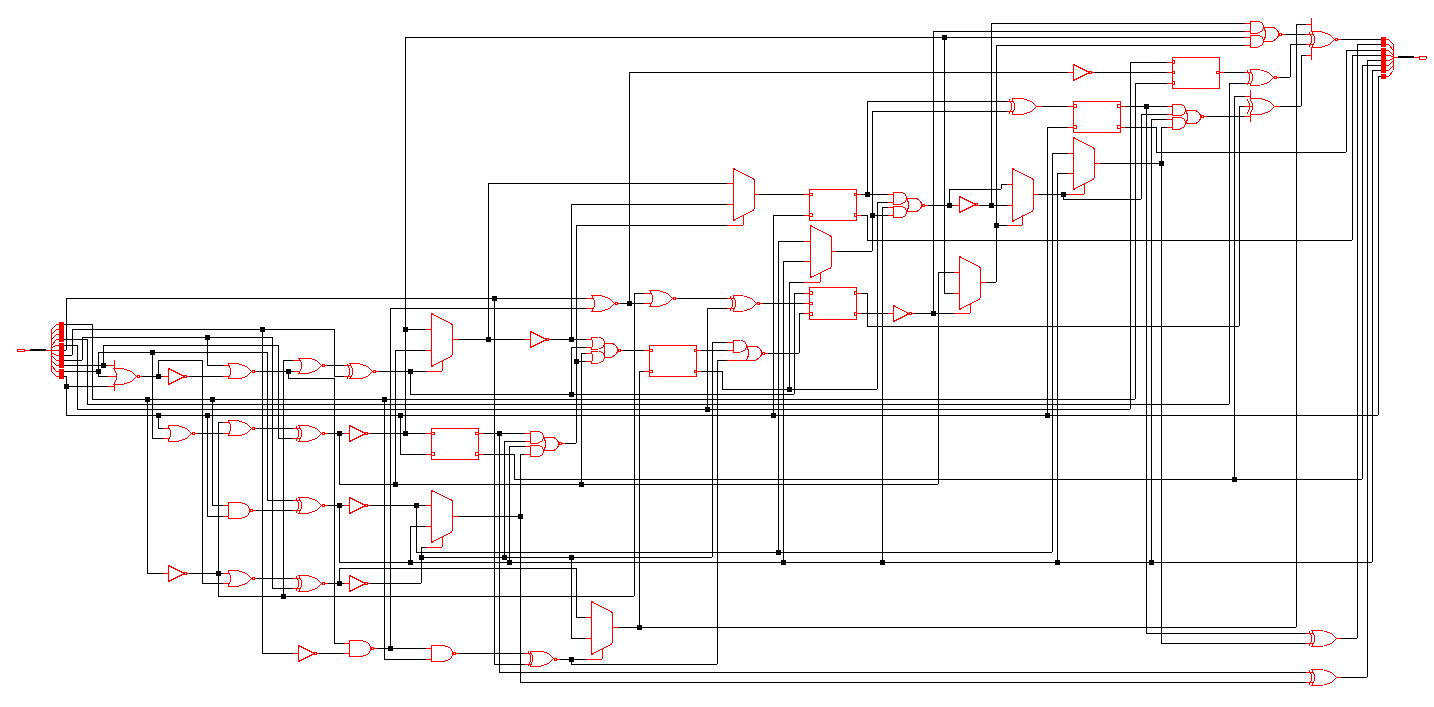
\includegraphics[width=1\textwidth]{img/Konstantenmultiplizierer_Encounter_sw.png}
  }
  \caption{12 Bit Konstantenmultiplizierer für $\frac{\sqrt{2}}{2} = 0,70711... \simeq 0,70703 = 010110101000_2$ in Encounter}
\end{figure}



\begin{table}[!ht]
 \caption{Vergleich Konstanten- mit regulärem Multiplizierer}
 \label{tab:VergleichMultiplizierer}
 \begin{tabular}{ccc}
 \hline
		& Konstantenmultiplizierer 	& regulärer Multiplizierer\\
  \hline	
  Gatter			& 43				& ? \\
  Inverter			& 10				& ? \\
  Summe				& 53				& ? \\
  Fläche (Prozess: 350nm)	& 4787 nm$^2$?			& ? \\
  \hline
 \end{tabular}
\end{table}


Der Ausgang hat so wie der Eingang 12 Bit, die niederwertigsten 12 Bit werden somit verworfen.

Auf Skript verweisen, mit dem ermittelt wurde, dass das die beste Annäherung an $\frac{\sqrt{2}}{2}$ ist.

Der vollständige Gate-Report befindet sich in Abschnitt \ref{src:rc_gate_report} auf Seite \pageref{src:rc_gate_report}



